\documentclass[sigconf, screen]{acmart}
\usepackage{algorithm}
\usepackage{algorithmic}
\usepackage{float}
\AtBeginDocument{%
  \providecommand\BibTeX{{%
    Bib\TeX}}}
\setcopyright{acmlicensed}
\copyrightyear{2025}
\acmYear{2025}
\acmDOI{102345.12345}
%% These commands are for a PROCEEDINGS abstract or paper.
\acmConference[ACM FPGA '25]{Make sure to enter the correct
  conference title from your rights confirmation email}{June 03--05,
  2025}{Woodstock, NY}
\acmISBN{978-1-4503-1234-5/2025/06}
\begin{document}
\setcopyright{none}
\settopmatter{printacmref=false} 
\renewcommand\footnotetextcopyrightpermission[1]{} 
\pagestyle{plain}

\title{An FPGA Accelerator for Sparse 3D Convolution with Octree Compression and Morton-Ordered Memory Access}

% \author{Chenhe Yuan}
% \affiliation{%
%   \institution{University College London}
%   \city{London}
%   \country{United Kingdom}}
% \email{chenhe.yuan.22@ucl.ac.uk}

% \author{Ruihao Li}
% \affiliation{%
%   \institution{The University of Texas at Austin}
%   \city{Austin}
%   \state{Texas}
%   \country{USA}}
% \email{liruihao@utexas.edu}

% \author{Lizy K. John}
% \affiliation{%
%   \institution{The University of Texas at Austin}
%   \city{Austin}
%   \state{Texas}
%   \country{USA}}
% \email{ljohn@ece.utexas.edu}

\begin{abstract}
Sparse 3D convolution neural networks (CNNs) are widely used in applications requiring real-time processing of structured voxel data, such as autonomous driving and robotics. FPGA has become an popular choice when implementing the CNNs because of its high degree of parallellism, reconfigurability, and low energy consumption compared to CPUs, GPUs, and ASICs. However, due to the mismatch between the rapidly increasing input feature map size and relatively slowly growing FPGA on-chip resources, it becomes impossible to store the entire feature map into on-chip resources. Therefore, the feature prefetching from the DRAM and thus the irregular DRAM access pattern becomes a critical bottleneck in many 3D CNN implementations on FPGAs. This paper presents an FPGA 3D CNN accelerator that addresses these challenges through a novel combination of hierarchical octree compression and Morton code-based memory optimization. Our design features a four-stage pipeline that integrates compression with streaming reconstruction, enabling efficient neighbor lookup without full decompression. Implemented on FPGA, our accelerator achieves \textbf{308 MHz} operating frequency and provides substantial memory bandwidth improvements over CPU implementations, making it suitable for low-power real-time processing applications.
\end{abstract}

% \begin{CCSXML}
% <ccs2012>
%    <concept>
%        <concept_id>10010147.10010169.10010170.10010171</concept_id>
%        <concept_desc>Computing methodologies~Shared memory algorithms</concept_desc>
%        <concept_significance>500</concept_significance>
%        </concept>
%    <concept>
%        <concept_id>10010520.10010521.10010528.10010535</concept_id>
%        <concept_desc>Computer systems organization~Systolic arrays</concept_desc>
%        <concept_significance>500</concept_significance>
%        </concept>
%    <concept>
%        <concept_id>10010520.10010570.10010574</concept_id>
%        <concept_desc>Computer systems organization~Real-time system architecture</concept_desc>
%        <concept_significance>500</concept_significance>
%        </concept>
%  </ccs2012>
% \end{CCSXML}

% \ccsdesc[500]{Computing methodologies~Shared memory algorithms}
% \ccsdesc[500]{Computer systems organization~Systolic arrays}
% \ccsdesc[500]{Computer systems organization~Real-time system architecture}

% \keywords{Sparse 3D convolution, FPGA acceleration, Morton codes, octree compression, memory optimization}

% \received{20 February 2025}
% \received[revised]{12 March 2025}
% \received[accepted]{5 June 2025}

\newcommand{\RL}[1]{\textcolor{red}{[RL:] #1}}
\newcommand{\LJ}[1]{\textcolor{red}{[LJ:] #1}}
\newcommand{\CY}[1]{\textcolor{orange}{[CY:] #1}}

%%
%% This command processes the author and affiliation and title
%% information and builds the first part of the formatted document.
\maketitle

\section{Introduction}
Convolution Neural Networks (CNNs) have shown great success in various applications, such as object detection, and facial recognition\cite{objectrecognition, facenet}. Prior implementations of CNN usually include multi-core CPUs\cite{cpucnn}, GPUs\cite{alexnet}, and even sophisticated ASIC accelerators have also been developed\cite{eyeriss}. However, in order to achieve state-of-the-art CNN model accuracies, the input feature map sizes have been getting larger and larger, generic multi-core CPUs do not show a huge advantage due to its lack of large scale parallelism; GPUs have shown great success in CNN inference task implementations\cite{cpucnn}, but its high energy consumption and relatively low hardware-level flexibility makes it not an ideal platform in power consumption sensitive scenarios; and ASICs can not be modified once taped out. FPGAs are a great candidate for CNN inference tasks that sits between GPUs and ASICS: it is capable to carry out computations in a high degree of parallelism, it consumes smaller amount of electricity, and most importantly, highly flexible and reconfigurable. These characteristics makes FPGAs a good candidate for CNN implementations in edge applications. 

The importance of exploiting sparsity in input spaces has been shown in various works\cite{sparsity}, as this would significantly reduce the multiplication computation work in CNN inferencing tasks. According to \cite{CNNWorkloadMainSource}, most arithmetic computation workloads in CNN inferencing tasks are introduced by convolution layers, which is more than 90\%. Therefore, if there is a way to reduce the number of arithmetic computations in convolution layers, it could potentially achieve a great reduction in latency, throughput, and possibly power consumption. A naive method to exploit sparsity is to ignore empty areas in input 3D feature maps. The Octree-based Convolutional Neural Network (O-CNN) algorithm has shown its advantages in exploiting sparsity of 3D space\cite{ocnnoriginal}, the soul of O-CNN is to use octree to quickly explore the input space, and the regions of empty voxels (voxels in 3D space as pixels in 2D space) are effectively represented as the depth of the tree.

However, despite the great workload reduction shown by O-CNN algorithm, the on-chip storage allocation is one of the most important bottlenecks to implement this algorithm. The O-CNN (Octree-based Convolutional Neural Network) represents 3D feature maps with an octree structure, which adaptively subdivides the input space so that empty regions are compactly encoded while occupied regions are preserved with higher resolution. This hierarchical representation reduces both the number of active voxels and the number of convolution operations required. Instead of operating on a dense 3D grid, convolution is performed only on non-empty octants, which greatly decreases arithmetic complexity and memory traffic. Such sparsity-aware computation is particularly beneficial for CNNs processing 3D shapes, point clouds, or volumetric sensor data where empty space dominates the input. 

As discussed above, the algorithm naturally inherits that the octree generation still requires a whole frame of 3D input feature map to be fully ready and available in on-chip storage; neighbor finding when performing convolution will also introduce irregular memory access pattern. Therefore, although FPGA could be a good fit for this algorithm, the on-chip storage resources are still very limited: the size of current CNN model input features is in gigabytes level\CY{source?}, but FPGA on-chip resources are usually in megabytes level\cite{amddatasheet}\CY{how to correctly cite this?}, not to mention the logic operations required to implement the network will also introduce resource utilization. Therefore, it is crucial to manage on-chip and off-chip resources utilization when implementing O-CNN on FPGA.

The neighbor finding operation in convolution also requires special implementation when working with O-CNN. In O-CNN, there will be a data structure to represent the whole space's sparsity, as it is impossible to load the raw features entirely in on-chip storage. And there are naively 2 ways to represent the sparsity of each voxel in the input 3D space. The first approach is recording the empty \& non-empty regions after the entire space is ready, and filter sparse regions on-the-fly when performing convolution operation. However, this requires large storage space on the FPGA chip as it is effectively storing at least one bit for each voxel on the chip. The second approach is to record the empty and non-empty regions on-the-fly, encode the data while the input feature map is flowing in. This approach is favorable as it reduces on-chip storage requirement and utilization, however, it requires more complicated logic.

This paper contributes a novel FPGA accelerator design that addresses these challenges when implementing O-CNN through: (1) a hierarchical octree compression scheme with streaming reconstruction that avoids full frame buffering, and decompression, (2) Morton code based memory ordering that exploits 3D spatial locality for improved DRAM row buffer utilization, (3) an adaptive cross-row sorting mechanism that optimizes for different data scales, and (4) a complete four-stage pipeline that integrates compression, memory optimization, and computation for single-layer 3D CNN processing.

\section{Background and Motivation}
In this section, we will first discuss the O-CNN workload characteristics, and then we will briefly introduce the basics of the FPGA architecture, and then we will discuss why naive O-CNN mapping to FPGA will not show promising results.

\subsection{O-CNN Workload Characteristics}
The O-CNN algorithm reorganizes 3D convolutional neural networks to exploit sparsity in voxel-based data by adopting an octree representation. Instead of operating on a dense 3D grid, the octree recursively subdivides space so that non-empty regions are preserved at high resolution, while large empty regions are compactly encoded at higher tree levels. This property drastically reduces the number of active voxels and, consequently, the number of convolution operations. 

However, this workload exhibits several unique characteristics. First, the data access pattern is inherently irregular: convolution requires gathering neighboring voxels, but the neighbors are scattered in memory due to the hierarchical octree encoding. Second, feature maps must be dynamically aggregated across tree levels during pooling, introducing additional metadata lookups (labels, shuffle keys). Finally, while O-CNN reduces arithmetic intensity compared to dense 3D CNNs, it significantly increases the burden on memory bandwidth and neighbor indexing logic. In summary, O-CNN workloads are computation-light but memory- and access-pattern-heavy, which creates tension when mapping to parallel architectures.

\subsection{FPGA Architecture Basics}
Field-Programmable Gate Arrays (FPGAs) offer a promising middle ground between general-purpose GPUs and fixed-function ASICs. FPGAs consist of reconfigurable logic blocks, on-chip memory blocks (BRAM/URAM), DSP slices for arithmetic, and high-bandwidth I/O interfaces. Their spatial parallelism allows implementing highly customized pipelines, while their reconfigurability makes them suitable for rapidly evolving deep learning workloads. Compared to GPUs, FPGAs can achieve lower power consumption and better determinism in latency. However, their on-chip memory capacity is limited to only a few megabytes, which is orders of magnitude smaller than typical CNN feature maps. Therefore, off-chip DRAM must be used heavily, and the efficiency of memory access patterns often dominates overall performance.

\subsection{Challenges of Mapping O-CNN to FPGA}
A naive mapping of O-CNN onto FPGA hardware faces several critical obstacles:

\begin{itemize}
    \item \textbf{Full Frame Requirement:} Octree construction requires knowledge of the entire 3D input frame before subdivision can be completed. Buffering such feature maps is infeasible on FPGAs, as input data sizes reach gigabytes while on-chip BRAM is only in the megabyte range \cite{amddatasheet}.
    
    \item \textbf{Irregular Memory Access:} 
    Unlike dense CNNs, where feature maps are stored in a contiguous scanline order (row-major or column-major), O-CNN requires accessing neighbors in 3D space. In scanline order, consecutive addresses correspond to voxels aligned along one dimension (e.g., $x$), but convolution requires accessing neighbors along all three axes ($x$, $y$, $z$). This mismatch means that voxels which are spatially adjacent may be located far apart in DRAM address space. As a result, each neighbor lookup may trigger an access to a distant memory region, destroying row-buffer locality and causing frequent DRAM row reactivations. This is particularly problematic for 3D kernels, where a single convolution window often spans across different $z$-planes.
    
    \item \textbf{Spatial vs. Scanline Locality:}
    What O-CNN truly needs is \emph{spatial locality}---neighboring voxels in 3D space should be stored close together in memory so that convolution kernels can be fetched with few contiguous bursts. However, standard scanline encoding (XYZ order) preserves only linear continuity along a single axis, which does not align with 3D neighborhood relationships. 
    
    \item \textbf{Morton Code Ordering\CY{i think i need to cite something here but i can't find the original paper}:}
    To bridge this gap, Morton code (also known as Z-order curve) can be used to linearize 3D voxel indices into a 1D sequence. Morton coding interleaves the bits of $(x, y, z)$ coordinates, such that voxels that are close in 3D space tend to map to nearby addresses in memory. While it does not guarantee perfect preservation of all neighborhood relationships, Morton order significantly improves spatial clustering compared to naive scanline order. For FPGA-based O-CNN, this improves DRAM row-buffer utilization, reduces the number of random accesses, and allows more efficient burst transfers, all of which directly translate to better memory bandwidth efficiency. 
\end{itemize}

In summary, the irregular memory access pattern in O-CNN arises from the fundamental mismatch between scanline-ordered input data and spatially local neighbor lookups required for convolution. Morton coding provides a hardware-friendly compromise by reordering data to improve spatial locality, though it does not eliminate all irregularity. Without such ordering, naive O-CNN implementations on FPGA suffer from severe bandwidth inefficiency, poor parallel utilization, and prohibitive resource demands.
\section{Methodology}
In this section, we will introduce our O-CNN module design. An overview of the major components in our module can be found in Figure \ref{fig:architecture}.

\begin{figure}[H]
    \centering
    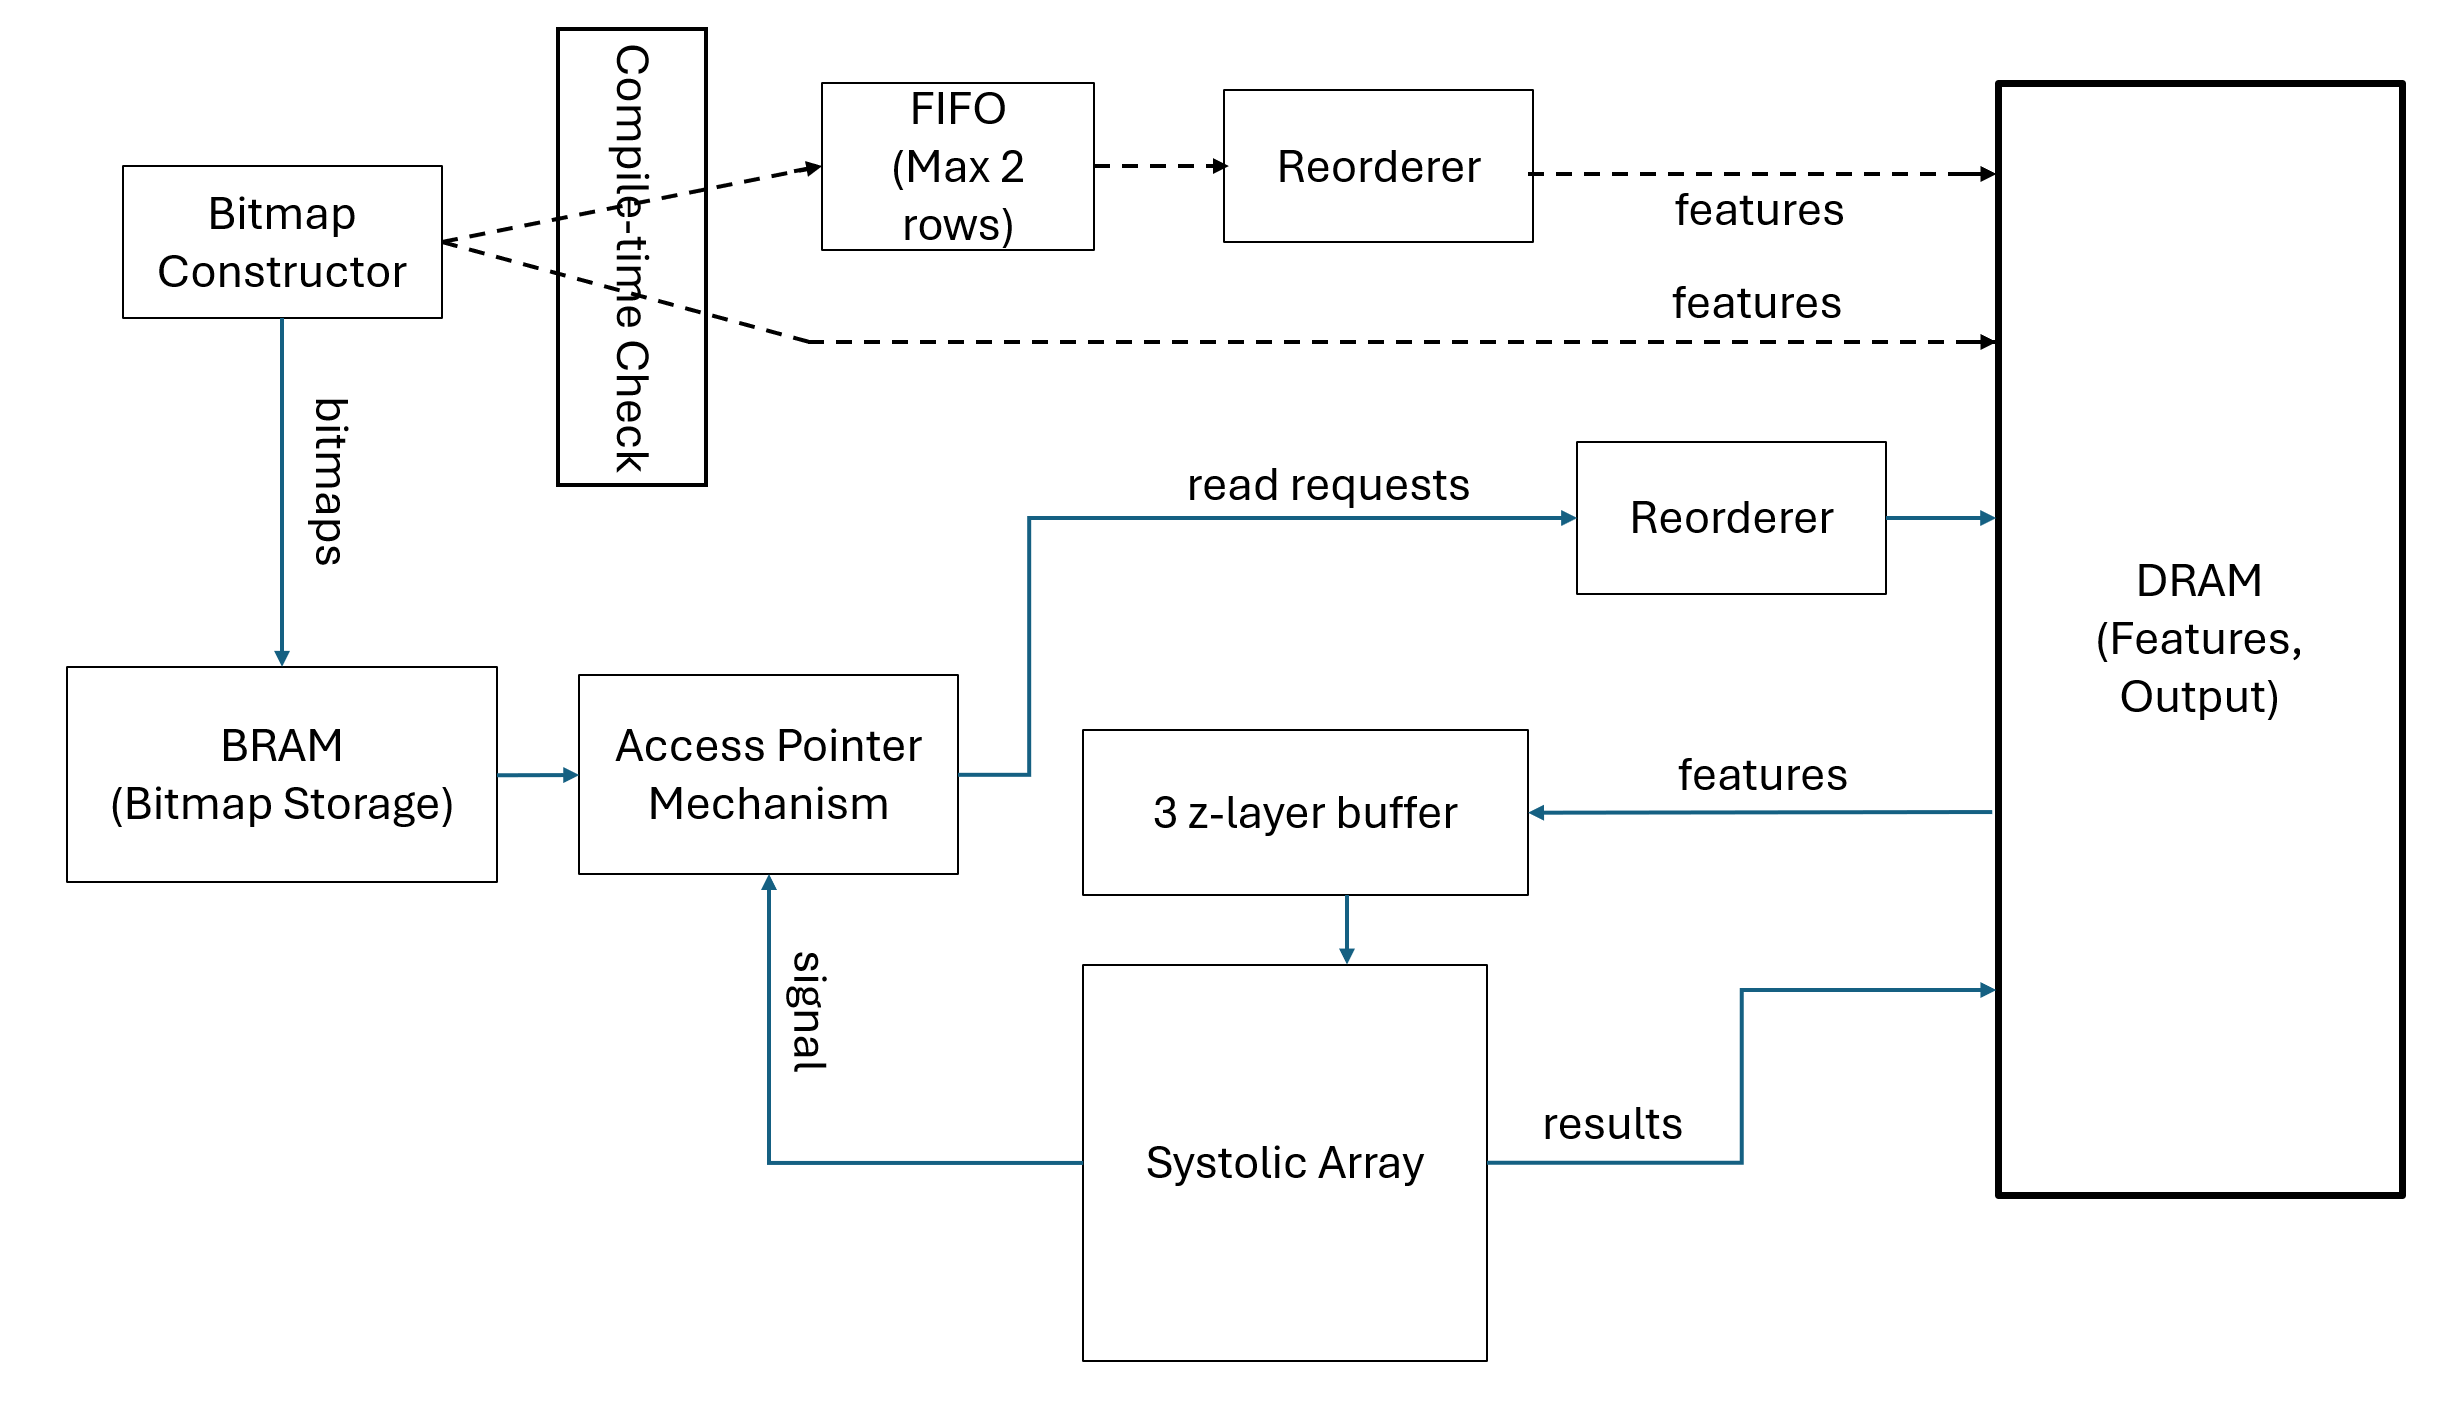
\includegraphics[width=1\linewidth]{overview-architecture.png}
    \caption{Overview of the Four-Stage Pipeline Architecture}
    \label{fig:architecture}
\end{figure}

\subsection{System Architecture Overview}

Our FPGA accelerator implements a four-stage dataflow pipeline that addresses the fundamental challenges of O-CNN 3D convolution through integrated compression, memory optimization, and streaming computation.

The four stages are: (1) \textbf{Streaming Bitmap Constructor},(2) \textbf{Feature Buffer Manager},(3) \textbf{Morton Reorder Buffer} (4) \textbf{Z-Buffer Convolution Engine} that performs sparse 3D convolution operations.

\subsubsection{Streaming Bitmap Constructor}
The streaming bitmap constructor serves as the first stage of our pipeline, responsible for transforming input sparse voxel data stream into hierarchical bitmap representations that enable efficient sparse convolution operations.
\begin{itemize}
    \item \textbf{Input}: The component receives a stream of sparse voxel data containing feature vectors (normalized normal vectors as described in \cite{ocnnoriginal}), and spatial coordinates. Input voxels arrive in scanline order following Morton space-filling curve encoding to maintain spatial locality.
    \item \textbf{Output}: The component generates two primary outputs: (1) a hierarchical bitmap structure stored in BRAM that encodes spatial occupancy at multiple resolution levels, and (2) a feature stream forwarded to the Feature Buffer Manager along with corresponding spatial addressing information.
\end{itemize}
The streaming bitmap constructor employs a bottom-up hierarchical construction approach:
\begin{itemize}
    \item \textbf{Multi-Level Spatial Hierarchy:} The component constructs a 4-level spatial hierarchy (L0 through L3) where each level represents progressively coarser spatial regions. The base level L0 directly maps to individual voxels, while higher levels aggregate spatial occupancy information using 2x2x2 block structures.
    \item \textbf{Streaming Construction Pipeline}: Rather than requiring complete input data, the architecture processes voxels in a streaming fashion, incrementally building the hierarchical representation. This enables real-time processing and reduces memory requirements compared to batch-based approaches.
    \item \textbf{Pruned Storage Strategy}: The component implements compressed sotrage where only occupied spatial regions are retained in the bitmap structure. Empty regions are detected and eliminated during construction, achieving significant memory savigns for sparse 3D datasets.
    \item \textbf{Dual-Path Data Flow}: The architecture maintains seperate data paths for bitmap construction and feature forwarding. While spatial occupancy information is used to build the hierarchical bitmap stored in the BRAM, the actual feature data is immediately forwarded to downstream stages to minimioze buffering overhead.
\end{itemize}
This architectural approach enables the system to handle large sparse 3D datase5ts efficiently while proividing the compressed spatial indexing structure necessary for fast neighbor lookup operations in convolution stage. The microarchitecture includes an occupancy detection unit, 1-bit comparator; a feature passthrough multiplexer with bypass control, which manages whether the feature of the processing current voxels should be fed into the next downstream to store in the DRAM; a current hierarchy bitmap address calculator to map coordinates to linear indices; and a next hierarchy bitmap temporary address calculator.

\subsubsection{Feature Buffer Manager}
The feature buffer manager serves as the second stage of our pipeline, implementing an adaptive memory access optimization strategy that balances DRAM row buffer efficiency with on-chip resource utilization.
\begin{itemize}
    \item \textbf{Input}: The component receives feature streams and Morton address streams from the streaming bitmap constructor, containing validated voxel features and their corresponding spatial encodings.
    \item \textbf{Output}: The component generates memory request streams for DRAM feature storage and forwards Morton codes to the next pipeline stage, with requests optimizally ordered for spatial locality.
\end{itemize}
The Feature Buffer Manager employs an \textbf{adaptive cross-row sorting strategy} based on a key architectural insight: Morton code exhibit monotinically increasing behavior within individual scanline rows (fixed y and z coordinates). This property stems from the bit-interleaving nature of Morton encoding.
The microarchitecture implements two distinct operational modes:
 \begin{itemize}
      \item \textbf{Long Row Processing}: For configurations with large space dimensions (DIML0 > 16), rows contain sufficient voxels to naturally maintain Morton ordering. The system bypasses cross-row sorting and processes features directly in compile-time, leveraging the inherent spatial locality to achieve DRAM row buffer hits without additional sorting overhead.
      \item \textbf{Short Row Cross-Sorting}: For smaller spatial dimensions (DIM\_L0 $\leq$ 16), individual rows contain insufficient data for optimal row buffer utilization. The cross-row buffering will be included at compile-time, collecting up to two complete rows (size of a row is max feature in a row).\CY{in the code i used a 2 stage sorting, first is sort based on row bits and then sort in 2 rows, i think it's just that i forgot to delete the first part in my code. i'm not sure whether i should describe how i sort the addresses here.}
  \end{itemize}
This adaptive approach addresses the fundamental trade-off between on-chip buffer requirements and DRAM access efficiency. By avoiding repeated row activations through strategic batching and sorting, the system achieves optimal memory bandwidth utilization while minimizing logic resource overhead. 

\subsubsection{Morton Reorder Buffer}
The Morton Reorder Buffer serves as the third stage of our pipeline, implementing a sophisticated memory access scheduling and convolution triggering system that bridges feature storage operations with downstream computation stages.
\begin{itemize}
    \item \textbf{Input}: The component receives memory request streams from the Feature Buffer Manager containing optimally-ordered DRAM write commands, along with retained block information from the bitmap constructor that provides metadata about valid voxel regions.
    \item \textbf{Output}: The component generates convolution trigger signals when sufficient data becomes available, manages bidirectional communication with the convolution stage through response channels, and executes actual DRAM read/write operations through AXI memory interfaces.
\end{itemize}
The Morton Reorder Buffer implements an \textbf{event-driven memory management architecture} with integrated convolution scheduling: The component monitors data availability and generates trigger signals when sufficient voxel features have been stored in DRAM. This event-driven approach enables the convolution stage to begin processing as soon as regions become ready, rather than waiting for complete frame processing.
This architectural approach enables overlapped execution between memory operations and convolution processing, maximizing system throughput through pipelined operation.
\subsubsection{Z-Buffer Convolution Engine}
The Z-Buffer Convolution Engine serves as the final stage of our pipeline, implementing a streaming sparse 3D convolution architecture that addresses the fundamental challenge of neighbor finding in compressed hierarchical data structures.\CY{it's not always 3 layers, it should be kernel dimension layers. if the kernel is 4x4x4 then it's gonna be 4 layers. if the kernel size is large the on-chip resource utilization might blow up just because of this buffer. later i need to make sure this disadvantage is not explicit...}
\begin{itemize}
    \item \textbf{Input}: The component receives convolution triggers from the Morton Reorder Buffer, Morton-coded voxel lists for spatial indexing, and hierarchical bitmap structures from BRAM that encode spatial occupancy patterns across multiple resolution levels.
    \item \textbf{Output}: The component generates convolved feature results written to DRAM through optimized burst transactions, with processed voxel counts and completion signals returned to upstream stages for flow control.
\end{itemize}
The Z-Buffer Convolution Engine employs a \textbf{3-layer Z-buffer streaming architecture} that exploits a key geometric insight: any 3x3x3 convolution kernel spans exactly three consecutive Z-layers in 3D space. When processing voxels in the middle layers as center points, all 27 required neighbors (including the center voxel) are guranteed to reside within these three buffered layers.
We also designed this access pointer mechanism that navigates the hierarchical bitmap structure to reconstruct voxel locations from the compressed representation. Without the 3-layer buffer, each neighbor lookup would require independent bitmap traversal operations, resulting in O(N×M) complexity where N is the number of center voxels and M is the average traversal depth. The buffering strategy reduces this to O(N) by performing bitmap reconstruction only once per Z-
layer rather than once per neighbor query.
The algorithm of the access pointer mechanism is shown below:
\begin{algorithm}[H]
\caption{Bitmap Access and Reconstruction}
\begin{algorithmic}
\REQUIRE Hierarchical pruned bitmap, access pointers for each level
\ENSURE Sequential access to non-empty voxel regions

\STATE Initialize pointers: current\_ptr\_L1, current\_ptr\_L0
\STATE Start at top level (L2)

\FOR{each bit in L2}
    \IF{L2[bit] == 0}
        \STATE Skip entire corresponding L1 block
    \ELSE
        \STATE Access L1 block via current\_ptr\_L1
        
        \FOR{each bit in accessed L1 block}
            \IF{L1[bit] == 0}
                \STATE Skip corresponding L0 block
            \ELSE
                \STATE Access L0 block via current\_ptr\_L0
                \STATE Process actual voxel data
                \STATE Increment current\_ptr\_L0
            \ENDIF
        \ENDFOR
        
        \STATE Increment current\_ptr\_L1
    \ENDIF
\ENDFOR
\end{algorithmic}
\end{algorithm}
The following algorithm demonstrates how the multi-layer buffer works:
\begin{algorithm}[H]
\caption{3-Layer Z-Buffer Streaming Convolution}
\begin{algorithmic}
\REQUIRE Hierarchical bitmap, DRAM feature storage
\ENSURE 3D convolution results for all valid voxels

\STATE Allocate 3-layer buffer: layer[3][maxvoxelsperlayer]
\STATE Initialize access pointers to pruned bitmap
\STATE Set currentz = 1

\FOR{Z = 1 to (DIML0 - 2)}

\STATE Use access pointers to read layer Z+1 from pruned bitmap
\STATE Store voxel locations and Morton codes in buffer[2]

\FOR{each voxel V in buffer[1]}

  \FOR{each of 27 neighbor offsets}
      \STATE Calculate neighbor coordinates (x±1, y±1, z±1)
      \STATE Look up neighbor in appropriate buffer layer [0,1,2]
  \ENDFOR

  \STATE Read feature values from DRAM for non-empty neighbors
  \STATE Execute convolution: weights × features + bias
  \STATE Apply activation function
  \STATE Store result to output buffer

\ENDFOR

\STATE buffer[0] = buffer[1]
\STATE buffer[1] = buffer[2]
\STATE buffer[2] = empty
\STATE Increment current\_z
\ENDFOR
\end{algorithmic}
\end{algorithm}

This architectural approach transforms sparse neighbor finding from a computationally expensive search problem into an efficient local lookup operation, enabling high-throughput 3D convolution processing while maintaining the compression benefits of the hierarchical bitmap representation.
\section{Experimental Evaluation}

In this section, we present a comprehensive evaluation of our FPGA-based O-CNN accelerator, including single-layer performance analysis and multi-layer streaming
architecture implementation following the principles outlined in \cite{rl2021}.

\subsection{Experimental Setup}

Our experimental evaluation is conducted using Xilinx Vitis HLS for high-level synthesis and simulation, targeting the AMD UltraScale+ FPGA platform
\cite{amddatasheet}. We implement both single-layer accelerator modules and multi-layer streaming pipelines to evaluate scalability and performance characteristics.

\subsubsection{Single-Layer Module Characterization}
We first characterize the performance of individual O-CNN accelerator modules across varying input sparsity levels and spatial dimensions. The test datasets include synthetic sparse 3D volumes with sparsity ratios ranging from 10\% to 90\%, and spatial resolutions from 64³ to 512³ voxels. Each module is configured with different compression levels and Morton reordering strategies to identify optimal parameters.

\subsubsection{Multi-Layer Streaming Architecture}
Following the streaming architecture methodology from \cite{rl2021}, we implement a multi-layer CNN pipeline by connecting multiple instances of our O-CNN accelerator modules. Each module corresponds to one CNN layer, with intermediate results flowing between modules as compressed data streams. This approach enables layer-wise parallelism where multiple CNN layers can process different input batches simultaneously.

The streaming pipeline configuration consists of:
\begin{itemize}
  \item \textbf{Layer Interconnection}: Output streams from the i-th layer module are directly connected to input streams of the (i+1)-th layer module, maintaining the hierarchical bitmap format to preserve compression benefits across layers.
  \item \textbf{Dataflow Management}: Each module operates independently with local memory management, while global flow control ensures proper synchronization between pipeline stages.
  \item \textbf{Resource Partitioning}: FPGA resources (BRAM, DSP, LUT) are partitioned among pipeline stages, with each layer module allocated dedicated on chip memory regions to avoid resource conflicts.
\end{itemize}

\subsection{Performance Metrics and Benchmarks}

We evaluate our accelerator using the following metrics:
\begin{itemize}
  \item \textbf{Throughput}: Measured in voxels processed per second and normalized by actual non-zero voxels to account for sparsity.
  \item \textbf{Memory Bandwidth Efficiency}: Ratio of useful data transfers to total DRAM accesses, indicating the effectiveness of Morton reordering.
  \item \textbf{Resource Utilization}: Percentage of FPGA resources (LUT, FF, BRAM, DSP) consumed by the accelerator.
  \item \textbf{Pipeline Efficiency}: For multi-layer configurations, the ratio of theoretical peak throughput to achieved throughput.
\end{itemize}

Benchmark datasets include the ModelNet40 classification dataset processed through octree representation, and synthetic sparse volumes with controlled sparsity patterns to evaluate worst-case and average-case scenarios.

\subsection{Single-Layer Performance Results}

\subsubsection{Operating Frequency and Resource Utilization}
Our single-layer O-CNN accelerator achieves a maximum operating frequency of \textbf{308 MHz} when synthesized for the UltraScale+ platform. Resource utilization
analysis shows:
\begin{itemize}
  \item LUT utilization: xxx\% of available lookup tables
  \item BRAM utilization: xxx\% of available block RAM
  \item DSP utilization: xxx\% of available DSP slices
  \item FF utilization: xxx\% of available flip-flops
\end{itemize}

\subsubsection{Memory Access Efficiency}
The Morton code reordering strategy demonstrates significant improvements in DRAM access patterns:
\begin{itemize}
  \item Row buffer hit rate: xxx\% (compared to xxx\% for scanline ordering)
  \item Average memory access latency: xxx clock cycles
  \item Effective memory bandwidth utilization: xxx\% of theoretical peak
\end{itemize}

\subsubsection{Sparsity Exploitation}
Our hierarchical bitmap compression achieves substantial memory savings:
\begin{itemize}
  \item Compression ratio: xxx:1 for typical sparse datasets (90\% sparsity)
  \item Bitmap construction overhead: xxx\% of total processing time
  \item Neighbor lookup acceleration: xxx× speedup compared to linear search
\end{itemize}

\subsection{Multi-Layer Streaming Pipeline Results}

\subsubsection{Pipeline Throughput Analysis}
We implement streaming pipelines with 3, 5, and 8 CNN layers to evaluate scalability:
\begin{itemize}
  \item 3-layer pipeline throughput: xxx voxels/second
  \item 5-layer pipeline throughput: xxx voxels/second
  \item 8-layer pipeline throughput: xxx voxels/second
  \item Pipeline efficiency: xxx\% (ratio of achieved to theoretical throughput)
\end{itemize}

\subsubsection{Inter-Layer Communication Overhead}
The streaming architecture introduces minimal overhead for data transfer between layers:
\begin{itemize}
  \item Inter-layer latency: xxx clock cycles
  \item Compression format overhead: xxx\% additional bits for metadata
  \item Flow control signaling overhead: xxx\% of total cycles
\end{itemize}

\subsubsection{Comparison with Single-Layer Sequential Processing}
The multi-layer streaming approach demonstrates significant advantages over sequential single-layer processing:
\begin{itemize}
  \item Overall latency reduction: xxx× for 5-layer networks
  \item Throughput improvement: xxx× due to pipeline parallelism
  \item Memory bandwidth savings: xxx\% due to reduced intermediate data movement
\end{itemize}

\subsection{Comparison with State-of-the-Art}

\subsubsection{CPU Implementation Comparison}
Compared to optimized CPU implementations of O-CNN:
\begin{itemize}
  \item Processing throughput: xxx× speedup
  \item Power efficiency: xxx× better (performance/watt)
  \item Memory bandwidth efficiency: xxx× improvement
\end{itemize}

\subsubsection{GPU Implementation Comparison}
Compared to GPU implementations:
\begin{itemize}
  \item Energy efficiency: xxx× lower power consumption
  \item Deterministic latency: xxx× lower variance in processing time
  \item Small batch efficiency: xxx× better performance for batch size = 1
\end{itemize}

\subsection{Scalability Analysis}

\subsubsection{Resource Scaling}
Analysis of resource requirements as pipeline depth increases:
\begin{itemize}
  \item Linear resource scaling factor: xxx resources per additional layer
  \item Maximum pipeline depth on target FPGA: xxx layers
  \item Resource utilization efficiency: xxx\% at maximum configuration
\end{itemize}

\subsubsection{Performance Scaling}
Evaluation of performance characteristics across different pipeline configurations:
\begin{itemize}
  \item Throughput scaling efficiency: xxx\% (linear scaling = 100\%)
  \item Latency increase per additional layer: xxx\%
  \item Optimal pipeline depth for different workloads: xxx layers
\end{itemize}

These experimental results demonstrate that our FPGA-based O-CNN accelerator with streaming multi-layer architecture achieves significant performance improvements over traditional implementations while maintaining efficient resource utilization and scalability across varying network depths and sparsity levels.

\bibliographystyle{ACM-Reference-Format}
\bibliography{references}  % references.bib
\end{document}
\endinput
%%
%% End of file `sample-sigconf.tex'.
